\documentclass{standalone}
\usepackage{tikz}
\usetikzlibrary{patterns, positioning}


\begin{document}
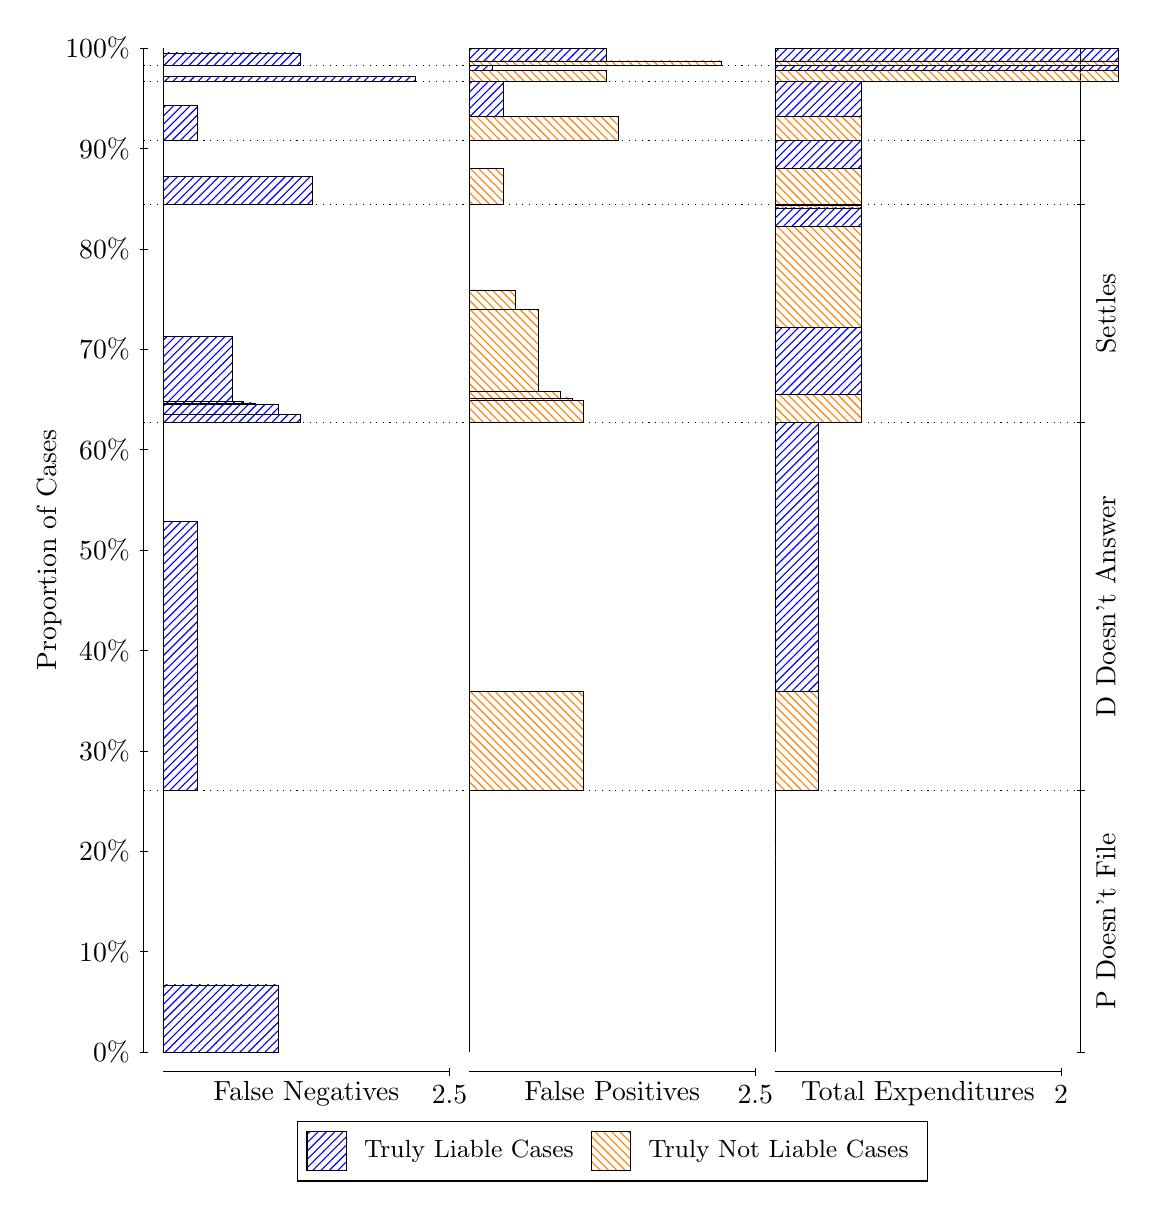
\begin{tikzpicture}
\draw[black, very thin] (1.5,1.75) -- (1.5,14.5);
\node[rotate=90, text=black, anchor=center] at (0.3, 8.125) {Proportion of Cases};
\draw[black, very thin] (1.45,1.75) -- (1.55,1.75);
\node[text=black, anchor=east] at (1.45, 1.75) {0\%};
\draw[black, very thin] (1.45,3.025) -- (1.55,3.025);
\node[text=black, anchor=east] at (1.45, 3.025) {10\%};
\draw[black, very thin] (1.45,4.3) -- (1.55,4.3);
\node[text=black, anchor=east] at (1.45, 4.3) {20\%};
\draw[black, very thin] (1.45,5.575) -- (1.55,5.575);
\node[text=black, anchor=east] at (1.45, 5.575) {30\%};
\draw[black, very thin] (1.45,6.85) -- (1.55,6.85);
\node[text=black, anchor=east] at (1.45, 6.85) {40\%};
\draw[black, very thin] (1.45,8.125) -- (1.55,8.125);
\node[text=black, anchor=east] at (1.45, 8.125) {50\%};
\draw[black, very thin] (1.45,9.4) -- (1.55,9.4);
\node[text=black, anchor=east] at (1.45, 9.4) {60\%};
\draw[black, very thin] (1.45,10.675) -- (1.55,10.675);
\node[text=black, anchor=east] at (1.45, 10.675) {70\%};
\draw[black, very thin] (1.45,11.95) -- (1.55,11.95);
\node[text=black, anchor=east] at (1.45, 11.95) {80\%};
\draw[black, very thin] (1.45,13.225) -- (1.55,13.225);
\node[text=black, anchor=east] at (1.45, 13.225) {90\%};
\draw[black, very thin] (1.45,14.5) -- (1.55,14.5);
\node[text=black, anchor=east] at (1.45, 14.5) {100\%};

\draw[black, very thin] (13.4,1.75) -- (13.4,14.5);
\draw[black, very thin] (13.35,1.75) -- (13.45,1.75);
\node[anchor=west] at (13.35, 1.75) {};
\draw[black, very thin] (13.35,5.0739) -- (13.45,5.0739);
\node[anchor=west] at (13.35, 5.0739) {};
\draw[black, very thin] (13.35,9.7424) -- (13.45,9.7424);
\node[anchor=west] at (13.35, 9.7424) {};
\draw[black, very thin] (13.35,12.515) -- (13.45,12.515);
\node[anchor=west] at (13.35, 12.515) {};
\draw[black, very thin] (13.35,13.325) -- (13.45,13.325);
\node[anchor=west] at (13.35, 13.325) {};
\draw[black, very thin] (13.35,14.074) -- (13.45,14.074);
\node[anchor=west] at (13.35, 14.074) {};
\draw[black, very thin] (13.35,14.276) -- (13.45,14.276);
\node[anchor=west] at (13.35, 14.276) {};
\draw[black, very thin] (13.35,14.5) -- (13.45,14.5);
\node[anchor=west] at (13.35, 14.5) {};

\draw[black, very thin, pattern color=blue, pattern=north east lines] (1.75,1.75) rectangle (3.2033,2.6018);
\draw[black, very thin, pattern color=orange, pattern=north west lines] (1.75,2.6018) rectangle (1.75,5.0739);
\draw[black, very thin, pattern color=blue, pattern=north east lines] (1.75,5.0739) rectangle (2.186,8.4851);
\draw[black, very thin, pattern color=orange, pattern=north west lines] (1.75,8.4851) rectangle (1.75,9.7424);
\draw[black, very thin, pattern color=blue, pattern=north east lines] (1.75,9.7424) rectangle (3.494,9.8452);
\draw[black, very thin, pattern color=blue, pattern=north east lines] (1.75,9.8452) rectangle (3.2033,9.9744);
\draw[black, very thin, pattern color=blue, pattern=north east lines] (1.75,9.9744) rectangle (2.9127,9.9933);
\draw[black, very thin, pattern color=blue, pattern=north east lines] (1.75,9.9933) rectangle (2.7673,10.009);
\draw[black, very thin, pattern color=blue, pattern=north east lines] (1.75,10.009) rectangle (2.622,10.833);
\draw[black, very thin, pattern color=orange, pattern=north west lines] (1.75,10.833) rectangle (1.75,12.515);
\draw[black, very thin, pattern color=blue, pattern=north east lines] (1.75,12.515) rectangle (3.6393,12.868);
\draw[black, very thin, pattern color=orange, pattern=north west lines] (1.75,12.868) rectangle (1.75,13.325);
\draw[black, very thin, pattern color=blue, pattern=north east lines] (1.75,13.325) rectangle (2.186,13.769);
\draw[black, very thin, pattern color=orange, pattern=north west lines] (1.75,13.769) rectangle (1.75,14.074);
\draw[black, very thin, pattern color=blue, pattern=north east lines] (1.75,14.074) rectangle (4.9473,14.136);
\draw[black, very thin, pattern color=orange, pattern=north west lines] (1.75,14.136) rectangle (1.75,14.276);
\draw[black, very thin, pattern color=blue, pattern=north east lines] (1.75,14.276) rectangle (3.494,14.438);
\draw[black, very thin, pattern color=orange, pattern=north west lines] (1.75,14.438) rectangle (1.75,14.5);
\draw[black, very thin, pattern color=orange, pattern=north west lines] (5.6333,1.75) rectangle (5.6333,4.2221);
\draw[black, very thin, pattern color=blue, pattern=north east lines] (5.6333,4.2221) rectangle (5.6333,5.0739);
\draw[black, very thin, pattern color=orange, pattern=north west lines] (5.6333,5.0739) rectangle (7.0867,6.3312);
\draw[black, very thin, pattern color=blue, pattern=north east lines] (5.6333,6.3312) rectangle (5.6333,9.7424);
\draw[black, very thin, pattern color=orange, pattern=north west lines] (5.6333,9.7424) rectangle (7.0867,10.028);
\draw[black, very thin, pattern color=orange, pattern=north west lines] (5.6333,10.028) rectangle (6.9413,10.056);
\draw[black, very thin, pattern color=orange, pattern=north west lines] (5.6333,10.056) rectangle (6.796,10.135);
\draw[black, very thin, pattern color=orange, pattern=north west lines] (5.6333,10.135) rectangle (6.5053,11.178);
\draw[black, very thin, pattern color=orange, pattern=north west lines] (5.6333,11.178) rectangle (6.2147,11.424);
\draw[black, very thin, pattern color=blue, pattern=north east lines] (5.6333,11.424) rectangle (5.6333,12.515);
\draw[black, very thin, pattern color=orange, pattern=north west lines] (5.6333,12.515) rectangle (6.0693,12.972);
\draw[black, very thin, pattern color=blue, pattern=north east lines] (5.6333,12.972) rectangle (5.6333,13.325);
\draw[black, very thin, pattern color=orange, pattern=north west lines] (5.6333,13.325) rectangle (7.5227,13.631);
\draw[black, very thin, pattern color=blue, pattern=north east lines] (5.6333,13.631) rectangle (6.0693,14.074);
\draw[black, very thin, pattern color=orange, pattern=north west lines] (5.6333,14.074) rectangle (7.3773,14.214);
\draw[black, very thin, pattern color=blue, pattern=north east lines] (5.6333,14.214) rectangle (5.924,14.276);
\draw[black, very thin, pattern color=orange, pattern=north west lines] (5.6333,14.276) rectangle (8.8307,14.338);
\draw[black, very thin, pattern color=blue, pattern=north east lines] (5.6333,14.338) rectangle (7.3773,14.5);
\draw[black, very thin, pattern color=orange, pattern=north west lines] (9.5167,1.75) rectangle (9.5167,4.2221);
\draw[black, very thin, pattern color=blue, pattern=north east lines] (9.5167,4.2221) rectangle (9.5167,5.0739);
\draw[black, very thin, pattern color=orange, pattern=north west lines] (9.5167,5.0739) rectangle (10.062,6.3312);
\draw[black, very thin, pattern color=blue, pattern=north east lines] (9.5167,6.3312) rectangle (10.062,9.7424);
\draw[black, very thin, pattern color=orange, pattern=north west lines] (9.5167,9.7424) rectangle (10.607,10.106);
\draw[black, very thin, pattern color=blue, pattern=north east lines] (9.5167,10.106) rectangle (10.607,10.949);
\draw[black, very thin, pattern color=orange, pattern=north west lines] (9.5167,10.949) rectangle (10.607,12.239);
\draw[black, very thin, pattern color=blue, pattern=north east lines] (9.5167,12.239) rectangle (10.607,12.471);
\draw[black, very thin, pattern color=orange, pattern=north west lines] (9.5167,12.471) rectangle (10.607,12.499);
\draw[black, very thin, pattern color=blue, pattern=north east lines] (9.5167,12.499) rectangle (10.607,12.515);
\draw[black, very thin, pattern color=orange, pattern=north west lines] (9.5167,12.515) rectangle (10.607,12.972);
\draw[black, very thin, pattern color=blue, pattern=north east lines] (9.5167,12.972) rectangle (10.607,13.325);
\draw[black, very thin, pattern color=orange, pattern=north west lines] (9.5167,13.325) rectangle (10.607,13.631);
\draw[black, very thin, pattern color=blue, pattern=north east lines] (9.5167,13.631) rectangle (10.607,14.074);
\draw[black, very thin, pattern color=orange, pattern=north west lines] (9.5167,14.074) rectangle (13.877,14.214);
\draw[black, very thin, pattern color=blue, pattern=north east lines] (9.5167,14.214) rectangle (13.877,14.276);
\draw[black, very thin, pattern color=orange, pattern=north west lines] (9.5167,14.276) rectangle (13.877,14.338);
\draw[black, very thin, pattern color=blue, pattern=north east lines] (9.5167,14.338) rectangle (13.877,14.5);
\draw[black, dotted] (1.5,5.0739) -- (13.4,5.0739);
\draw[black, dotted] (1.5,9.7424) -- (13.4,9.7424);
\draw[black, dotted] (1.5,12.515) -- (13.4,12.515);
\draw[black, dotted] (1.5,13.325) -- (13.4,13.325);
\draw[black, dotted] (1.5,14.074) -- (13.4,14.074);
\draw[black, dotted] (1.5,14.276) -- (13.4,14.276);
\draw[black, very thin] (1.75,1.5) -- (5.3833,1.5);
\node[text=black, anchor=north] at (3.5667, 1.5) {False Negatives};
\draw[black, very thin] (5.3833,1.45) -- (5.3833,1.55);
\node[text=black, anchor=north] at (5.3833, 1.45) {2.5};

\draw[black, very thin] (5.6333,1.5) -- (9.2667,1.5);
\node[text=black, anchor=north] at (7.45, 1.5) {False Positives};
\draw[black, very thin] (9.2667,1.45) -- (9.2667,1.55);
\node[text=black, anchor=north] at (9.2667, 1.45) {2.5};

\draw[black, very thin] (9.5167,1.5) -- (13.15,1.5);
\node[text=black, anchor=north] at (11.333, 1.5) {Total Expenditures};
\draw[black, very thin] (13.15,1.45) -- (13.15,1.55);
\node[text=black, anchor=north] at (13.15, 1.45) {2};

\node[text=black, centered, rotate=90] at (13.72, 3.4119) {P Doesn't File};
\node[text=black, centered, rotate=90] at (13.72, 7.4082) {D Doesn't Answer};
\node[text=black, centered, rotate=90] at (13.72, 11.129) {Settles};





\draw (7.449999999999999,1.5) node[draw=none] (baseCoordinate) {};
\begin{scope}[align=center]
        \matrix[scale=0.5, draw=black, below=0.5cm of baseCoordinate, nodes={draw}, column sep=0.1cm]{
            \node[rectangle, draw, minimum width=0.5cm, minimum height=0.5cm, pattern color=blue, pattern=north east lines] {}; &
            \node[draw=none, font=\small, text=black] (B) {Truly Liable Cases}; &
            \node[rectangle, draw, minimum width=0.5cm, minimum height=0.5cm, pattern color=orange, pattern=north west lines] {}; &
            \node[draw=none, font=\small, text=black] (B) {Truly Not Liable Cases}; \\
            };
\end{scope}

\end{tikzpicture}
\end{document}